% Template para o relatório final de estágio
% Autor: Fábio Engel de camargo

\documentclass{config/utfpr-style-estagio}
%comandos personalizados
\newboolean{temDedicatoria}
\setboolean{temDedicatoria}{false}

\newboolean{temAgradecimento}
\setboolean{temAgradecimento}{false}

\newboolean{temTabela}
\setboolean{temTabela}{true}

\newboolean{temFigura}
\setboolean{temFigura}{true}


% Redefine formato de lista de tabelas e figuras
\renewcommand{\cftloftitlefont}{\hfill\Large\bfseries}
\renewcommand{\cftafterloftitle}{\hfill}
\renewcommand{\cftlottitlefont}{\hfill\Large\bfseries}
\renewcommand{\cftafterlottitle}{\hfill}

\renewcommand{\cfttoctitlefont}{\hfill\Large\bfseries} %Define Sumário centralizado
\renewcommand{\cftaftertoctitle}{\hfill\hfill}
\author{Nome do Aluno}
\title{Título do Trabalho}
\curso{Tecnologia em Sistemas para Internet}
\empresa{Nome da Empresa}
\cidade{Toledo}
\ano % Se ano diferente do ano corrente, informar \ano[XXXX]
\profTitulo{Dr.} %acrônimo do título do professor. Ex: Dr., MS..
\orientador{Nome do Orientador}
\titulo{Tecnólogo em Sistemas para Internet}
\avaliador{Nome do prof. Avaliador}
\supervisor{Nome do Supervisor}
\prae{Nome do prof. Responsável pelo Estágio}
\diaDefesa{00}
\mesDefesa{janeiro}

%Se optar por escrever a Dedicatória, defina o argumento como true e escreva o conteúdo como parâmetro em \dedicatoria.
\setboolean{temDedicatoria}{true} % define como falso por padrão
\dedicatoria{Dedico este trabalho a...}

%Se optar por escrever Agradecimentos, defina o argumento como true e escreva o conteúdo como parâmetro em \agradecimento..
\setboolean{temAgradecimento}{true}
\agradecimento{Agradeço primeiramente a...}

%Se o seu texto não possuir figuras, descomente o comando abaixo.
%\setboolean{temFigura}{false}

%Se o seu texto não possuir tabelas, descomente o comando abaixo.
%\setboolean{temTabela}{false}

\begin{document}
	\pretexto
	% define estilo do corpo do documento (capítulos e apêndices)
	\mainmatter
	\pagestyle{mainmatter}
	\chapter{Introdução}
\label{cap:introducao}
%=====================================================

Este Relatório de Estágio.....

\section{Exemplo de figura}

\begin{figure}[ht]
	\centering
	\caption{Exemplo de figura.}
	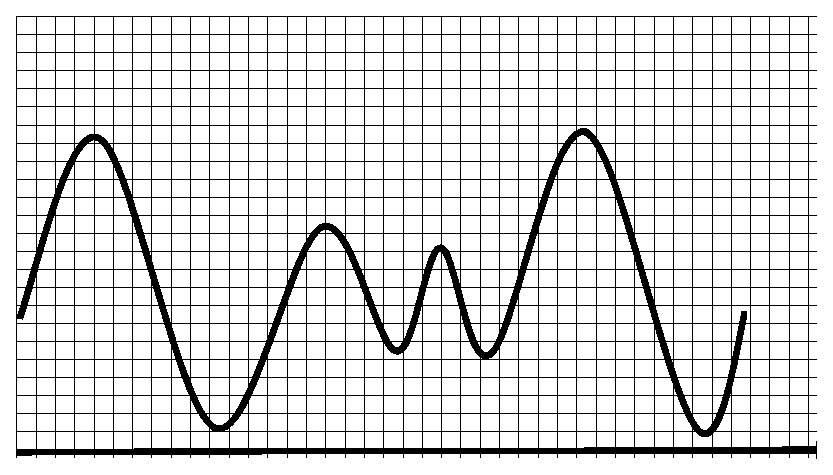
\includegraphics[width=0.5\textwidth]{fig/figexemplo.eps}
	\label{fig:figexemplo}
\end{figure}


\section{Exemplo de tabela}

\begin{table}[ht]
	\centering
	\caption{Exemplo de tabela.}
	\label{tab:exemplo}
	\begin{tabular}{|c|c|c|}
		\hline
		\textbf{Coluna 1} & \textbf{Coluna 2} & \textbf{Coluna 3} \\ \hline
		Linha 1 & Valor 1 & Valor 2 \\ \hline
		Linha 2 & Valor 3 & Valor 4 \\ \hline
	\end{tabular}
\end{table}

\section{Exemplos de citações}

Nesta seção são apresentados alguns exemplos de como realizar citações. Note que podem ser utilizados as macros \verb|\citet| e \verb|\cite|. A macro \verb|\citet| é utilizada para citar referências no formato de texto normal, em que o nome do autor (ou autores) e o ano da publicação são apresentados no texto. A macro \verb|\cite| é utilizada para citar referências entre parênteses, em que o nome do autor (ou autores) e o ano da publicação são apresentados dentro dos parênteses.

\subsection{Exemplo 1}
Neste ano, o Núcleo de Informação e Coordenação do Ponto BR (NIC.br), responsável pela administração e coordenação do domínio de topo ``.br'' da Internet, emitiu um alerta sobre a iminente escassez de endereços IPv4. Em 31 de janeiro, os últimos blocos disponíveis de endereços IPv4 foram distribuídos, incluindo para a região da América Latina e Caribe, da qual o Brasil faz parte. Estima-se que o Brasil ainda possua estoque de endereços IPv4 no padrão ``.br'' para distribuição por mais um ano, por meio do NIC.br \citep{nicbr2023IANA}.

\subsection{Exemplo 2}
O estudo de \citet{spanhol2015dataset} apresenta um conjunto de dados composto por 7.909 imagens de histopatologia de câncer de mama, obtidas de 82 pacientes, e disponíveis em uma plataforma pública. O conjunto de dados, disponibilizado em \url{http://web.inf.ufpr.br/vri/breast-cancer-database}, inclui imagens tanto benignas quanto malignas e é destinado à tarefa de classificação automatizada dessas imagens em duas classes. Essa ferramenta de diagnóstico auxiliado por computador pode ser valiosa para os clínicos. 

\subsection{Exemplo 3}

A utilização da lógica fuzzy combinada a técnicas analíticas pode ser uma abordagem eficaz para alcançar maior eficiência energética em dispositivos de redes de sensores sem fios (\textit{Wireless Sensor Networks} - WSNs). Essa abordagem propõe o uso de métodos eficientes de seleção de retransmissores para melhorar a vida útil da bateria, o desempenho e a eficiência energética das WSNs \cite{engel2013relay}.

\subsection{Exemplo 4}

Nos dias atuais, as tecnologias modernas de tecnologia da informação têm sido amplamente utilizadas com o objetivo de aprimorar a eficiência e o desempenho de sistemas de produção e de rede. Essas tecnologias, como Internet das Coisas (IoT), Redes de Funções Virtuais (NFV), Aprendizado de Máquina e outras, têm sido aplicadas em diversos contextos, desde manufatura aditiva (impressão 3D) até gerenciamento de redes de telecomunicações. Essas abordagens inovadoras visam obter ganhos significativos em termos de otimização de processos, monitoramento em tempo real, detecção de falhas, automação e tomada de decisões baseada em dados \cite{huff2020building,scheffel2021automated}. 


	\chapter{Do Local de Estágio}
\label{cap:localestagio}
%=====================================================

Descrever a empresa onde o estágio foi desenvolvido.
	\chapter{Do Plano De Estágio}
\label{cap:plano}
%=====================================================

Descrever o plano de estágio, as atividades definidas e os prazos estipulados.
	\chapter{Descrição e Análise das Atividades Desenvolvidas}
\label{cap:descricao}
%=====================================================

Neste capítulo o estagiário fala detalhadamente das atividades que desenvolveu ao longo do estágio, sendo fundamental que estabeleça a relação entre a teoria e a prática. Caso tenha feito estágio em mais de uma área, pode-se dividir este capítulo em subtítulos. 
O desenvolvimento é a parte principal e mais extensa, que contém a exposição ordenada e pormenorizada do assunto, onde o estagiário apresenta as atividades desenvolvidas durante o estágio. Podem ser colocados desenhos, fotografias, gráficos, mapas, organogramas, fluxogramas, quadros, tabelas e figuras para melhor ilustração e comprovação das atividades desenvolvidas.

	\chapter{Conclusão}
\label{cap:conclusao}
%=====================================================

Concluir o relatório com uma pequena retomada das principais atividades desenvolvidas analisando a respectiva contribuição à sua formação profissional. Os pontos fortes e fracos do estágio.
	\chapter{Considerações Finais}
\label{cap:consideracoes}
%=====================================================

Esta é a parte final do Relatório de Estágio, na qual o estagiário deve apresentar as últimas considerações sobre seu estágio supervisionado.  % Este é opcional. Comentar, caso não deseje utilizar.
	
	%Só se coloca este item caso o estagiário tenha citado algum trecho de livro, apostila, artigo da Internet, enfim, qualquer item  publicado ou de acesso livre ao público em geral.
	\bibliography{bibliografia}
	
	%items opcionais. Comentar caso não utilize.
	\chapter{Apêndice}
\label{cap:apendice}

Neste capítulo colocam-se os itens criados pelo próprio estagiário, como por exemplo, uma ficha de cadastro de clientes, um programa de computador, um roteiro de entrevista, enfim, qualquer elemento criado pelo estagiário. Este capítulo não é obrigatório, desde que o estagiário não mencione no decorrer do seu relatório algo que ele tenha criado ou elaborado para a empresa concedente do estágio. Elemento opcional. 
É o texto ou documento com a finalidade de complementar sua argumentação, sem prejudicar o sentido do trabalho. O apêndice é identificado por letras maiúsculas consecutivas, travessão e pelos respectivos títulos. Excepcionalmente, utilizam-se letras maiúsculas dobradas, na identificação dos apêndices, quando esgotadas as letras do alfabeto.
	\chapter{Anexos}
\label{cap:anexos}

Elemento opcional, sendo um texto ou documento não elaborado pelo autor, que serve de fundamentação, comprovação e ilustração. Os anexos são identificados por letras maiúsculas consecutivas, travessão e pelos respectivos títulos. Excepcionalmente, utilizam-se letras maiúsculas dobradas, na identificação dos anexos, quando esgotadas as 26 letras do alfabeto.
\end{document}
